\documentclass[
a4paper, 12pt, % Papierformat, Schriftgröße
titlepage, 		 % extra Titelseite statt einfacher Überschrift
twoside,			 % beidseitiger Druck
headsepline,	 % Trennlinie für die Kopfzeile
BCOR5mm,			 % Binderand 5 mm
idxtotoc, bibtotoc]{scrreprt}	% Index (soweit vorhanden) und Literaturliste weggelassen: bibtotoc
				       % im Inhaltsverzeichnis aufführen
% Dokumentenklasse ist aus dem KOMA-Script-Paket die SCRReprt-Klasse.

\usepackage{presentation}
\raggedbottom
% \usepackage{svg}
%%%%%%%%%%%%%%%%%%%%%%%%%%%%%%%%%
% Beginn des Dokumentes         %
%%%%%%%%%%%%%%%%%%%%%%%%%%%%%%%%%

\begin{document}
\section{Basics}
\begin{algorithm}\label{alg:SGD}
    \begin{algorithmic}[1]
        \caption{Stochastic gradient descent}
        \REQUIRE learning rate $\lambda$
        \ENSURE a trained neural network
        \STATE initialize the network, dataset and training parameters
        \WHILE{stopping criteria is not met}
            \STATE sample minibatch of $m$ examples ${x^{(1)}, ... ,x^{(n)}}$
            \STATE compute gradient estimate $\hat{g}=\frac{1}{m} \nabla_\theta \sum_i L(f(x^{(i)};\theta),y^{(i)})$
            \STATE apply parameter update $\theta=\theta-\lambda\cdot\hat{g}$
        \ENDWHILE
        \STATE \textbf{return: the trained network}
    \end{algorithmic}
\end{algorithm}

\begin{algorithm}
    \begin{algorithmic}[1]
        \caption{Stochastic gradient descent with Momentum}
        \REQUIRE learning rate $\alpha$
        \REQUIRE momentum parameter $m$
        \ENSURE a trained neural network
        \STATE initialize the network, dataset and training parameters
        \WHILE{stopping criteria is not met}
            \STATE sample minibatch of $m$ examples ${x^{(1)}, ... ,x^{(n)}}$
            \STATE compute gradient estimate $\hat{g}=\frac{1}{m} \nabla_\theta \sum_i L(f(x^{(i);\theta}),y^{(i)})$
            \STATE compute velocity update $v=m \cdot v - \alpha \hat{g}$
            \STATE apply parameter update $\theta=\theta-v$
        \ENDWHILE
        \STATE \textbf{return: the trained network}
    \end{algorithmic}
\end{algorithm}

\begin{figure}[h]\label{fig:Results_scheduler}
    \begin{center}
        \begin{tikzpicture}
            \begin{axis}[
            grid=major, 
            grid style={dashed,gray!30},
            xlabel=Epoch,
            ylabel=Validation Accuracy,
            %xticklabels={,,},
            ymin=0.80,
			xmin=-10,
			legend pos=south east,
            width=10cm,
            restrict x to domain=0:450]
            \addplot[mark=None, color=blue] 
				table[x=Step, y=Value, col sep=comma]{../paper/images/network_csv/baseline/MobileNetV2/MobileNetV2_baseline_validation_acuracy.csv};
				\addlegendentry{baseline}
            \addplot[mark=None, color=red] 
				table[x=Step, y=Value, col sep=comma]{../paper/images/network_csv/scheduler/MobileNetV2/MobileNetV2_scheduler_cosine_validation_acuracy.csv};
				\addlegendentry{SGD with Warm Restart}
			\end{axis}
        \end{tikzpicture}
    \end{center}
\end{figure}

\begin{figure}[h]\label{fig:Scheduler_lr}
    \begin{center}
        \begin{tikzpicture}
            \begin{axis}[
            grid=major, 
            grid style={dashed,gray!30},
            xlabel=Epoch,
            ylabel=Learning rate,
            %xticklabels={,,},
			xmin=-10,
            width=10cm,
            restrict x to domain=0:450
            ]
            \addplot[mark=None, color=blue] 
				table[x=Step, y=Value, col sep=comma]{../paper/images/network_csv/lr/MobileNetV2/run-mobileNetV2_scheduler_cosine_1-tag-lr.csv};
			\end{axis}
        \end{tikzpicture}
    \end{center}
\end{figure}


\section{Methods}
\begin{algorithm}\label{alg:Distance_Motivation}
    \begin{algorithmic}[1]
        \caption{Machine Learning with distancing}
        \REQUIRE a set of parameters $\theta$ and a dataset
        \ENSURE a assignment of $\theta$ which maximizes performance
        \STATE initialize the network, dataset and training parameters
        \FOR{$i \leftarrow 1$ \textbf{to} desired number of epochs}
            \STATE compute foward and backward pass of training data
            \STATE update parameter values with optimizer
        \ENDFOR
        \STATE create checkpoint we want to distance from
		\FOR{$i \leftarrow$ next epoch \textbf{to} end}
			\FOR{checkpoint \textbf{in} list of checkpoints}
			\STATE compute parameter update which increases the distance to checkpoint
			\ENDFOR
		\STATE update parameter values with optimizer
        \ENDFOR
        \STATE \textbf{return: the final assignment of $\theta$}
    \end{algorithmic}
\end{algorithm}

\begin{figure}[h!]\label{fig:Distance2D}
    \begin{center}
        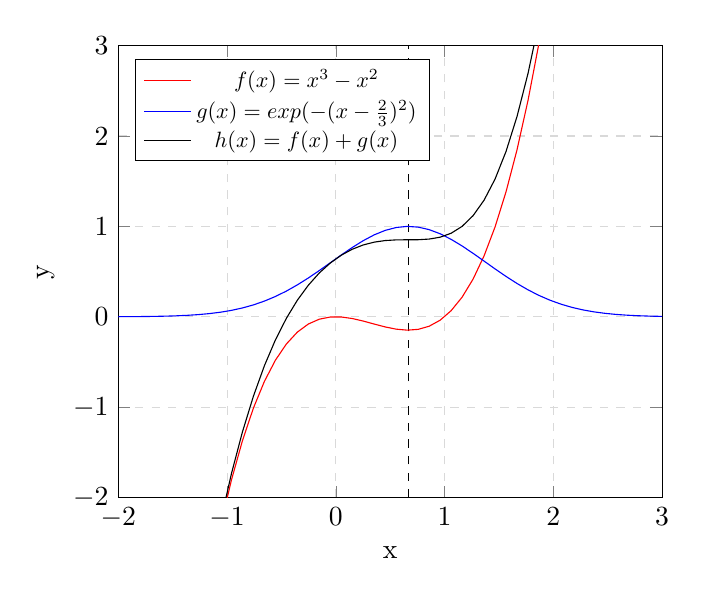
\begin{tikzpicture}
            \begin{axis}[
            grid=major, 
            grid style={dashed,gray!30},
            xlabel=x, % Set the labels
            ylabel=y,
            xmin=-2,
            xmax=3,
            xtick={-2,-1,0,1,2, 3},
            ymin=-2,
            ymax=3,
            samples=100,
            legend pos = north west,
            width=0.7\textwidth,
            legend style={nodes={scale=0.8, transform shape}}]
            \draw[dashed] ({axis cs:0.66666,0}|-{rel axis cs:0,0}) -- ({axis cs:0.66666,0}|-{rel axis cs:0,1});
            \addplot[color=red]{x^3-x^2};
            \addlegendentry{$f(x)=x^3-x^2$}
            \addplot[color=blue]{exp(-(x-2/3)^2)};
            \addlegendentry{$g(x)=exp(-(x-\frac{2}{3})^2)$}
            \addplot[color=black]{x^3-x^2+exp(-(x-2/3)^2)};
            \addlegendentry{$h(x)=f(x)+g(x)$}
            \end{axis}
         \end{tikzpicture}
    \end{center}
\end{figure}

\begin{algorithm}\label{alg:Distance_update}
    \begin{algorithmic}[1]
        \caption{Update step with distancing}
        \REQUIRE learning rate $\alpha$, distance hyperparameters $s$ and $\sigma$
        \ENSURE a trained neural network
        \STATE initialize the network, dataset and training parameters
        \WHILE{stopping criteria is not met}
            \STATE sample minibatch of $m$ examples ${x^{(1)}, ... ,x^{(n)}}$
            \STATE compute gradient estimate $\hat{g}=\nabla_\theta \frac{1}{m} \sum_i L(f(x^{(i)};\theta),y^{(i)})+ \frac{1}{c} \sum_c s_c\cdot distance(\theta , \theta_c)$
            \STATE apply parameter update $\theta=\theta-\alpha\cdot\hat{g}$
        \ENDWHILE
        \STATE \textbf{return: the trained network}
    \end{algorithmic}
\end{algorithm}

\section{results}

\begin{figure}[H]\label{fig:Results_baseline}
    \begin{center}
        \begin{tikzpicture}
            \begin{groupplot}[
                group style={
                group size=1 by 2,
                horizontal sep=10pt,
                vertical sep=40pt,
                group name=G},
                width=10cm,
            ]

            \nextgroupplot[
            grid=major, 
            grid style={dashed,gray!30},
            xlabel=Epoch,
            ylabel=Validation Accuracy,
            %xticklabels={,,},
			ymin=0.80,
			xlabel near ticks,
            xmin=-10]
            \addplot[mark=None, color=red] 
                table[x=Step, y=Value, col sep=comma]{../paper/images/network_csv/baseline/MobileNetV2/MobileNetV2_baseline_validation_acuracy.csv};
            \addplot[mark=None, color=blue] 
                table[x=Step, y=Value, col sep=comma]{../paper/images/network_csv/baseline/MobileNetV2/MobileNetV2_baseline_distance_validation_acuracy.csv};
            
            \nextgroupplot[
                grid=major, 
                grid style={dashed,gray!30},
                xlabel=Epoch,
                ylabel=Distance,
                %yticklabel pos=right,
                %xticklabels={,,},
				ylabel near ticks,
				xlabel near ticks,
				legend pos =south east]
                \addplot[mark=None, color=red] 
					table[x=Step, y=Value, col sep=comma]{../paper/images/network_csv/baseline/MobileNetV2/MobileNetV2_baseline_distance0.csv};
					\addlegendentry{baseline}
                \addplot[mark=None, color=blue] 
					table[x=Step, y=Value, col sep=comma]{../paper/images/network_csv/baseline/MobileNetV2/MobileNetV2_baseline_distance_distance0.csv};
					\addlegendentry{distance}
            \end{groupplot}
        \end{tikzpicture}
    \end{center}
\end{figure}


\begin{figure}[h]\label{fig:Results_strength}
    \begin{center}
        \begin{tikzpicture}
            \begin{groupplot}[
                group style={
                group size=1 by 2,
                horizontal sep=10pt,
                vertical sep=40pt,
                group name=G},
                width=10cm,
                restrict x to domain=0:200
            ]

            \nextgroupplot[
            grid=major, 
            grid style={dashed,gray!30},
            xlabel=Epoch,
            ylabel=Validation Accuracy,
            %xticklabels={,,},
            ymin=0.8,
            legend pos= south east,
			xmin=-10]
			\draw[dashed] ({axis cs:100,0}|-{rel axis cs:0,0}) -- ({axis cs:100,0}|-{rel axis cs:0,1});
            \addplot[mark=None, color=red] 
                table[x=Step, y=Value, col sep=comma]{../paper/images/network_csv/strength/MobileNetV2/MobileNetV2_strength_e1_validation_acuracy.csv};
            \addlegendentry{$s=0.1$}
            \addplot[mark=None, color=blue] 
                table[x=Step, y=Value, col sep=comma]{../paper/images/network_csv/baseline/MobileNetV2/MobileNetV2_baseline_distance_validation_acuracy.csv};
            \addlegendentry{$s=1$}
            \addplot[mark=None, color=orange] 
                table[x=Step, y=Value, col sep=comma]{../paper/images/network_csv/strength/MobileNetV2/MobileNetV2_strength_e2_validation_acuracy.csv};
            \addlegendentry{$s=10$}
            \addplot[mark=None, color=green] 
                table[x=Step, y=Value, col sep=comma]{../paper/images/network_csv/strength/MobileNetV2/MobileNetV2_strength_e3_validation_acuracy.csv};
			\addlegendentry{$s=100$}
			

            \nextgroupplot[
                grid=major, 
                grid style={dashed,gray!30},
                xlabel=Epoch,
                y label style={at={(-0.1,0.5)},anchor=south},
                ylabel=Distance,
                %yticklabel pos=right,
%                y label style={at={(axis description cs:0,0)},anchor=south},
                %xticklabels={,,},
                ylabel near ticks]
            \addplot[mark=None, color=red] 
                table[x=Step, y=Value, col sep=comma]{../paper/images/network_csv/strength/MobileNetV2/MobileNetV2_strength_e1_distance0.csv};
            \addplot[mark=None, color=blue] 
                table[x=Step, y=Value, col sep=comma]{../paper/images/network_csv/baseline/MobileNetV2/MobileNetV2_baseline_distance_distance0.csv};
            \addplot[mark=None, color=orange] 
                table[x=Step, y=Value, col sep=comma]{../paper/images/network_csv/strength/MobileNetV2/MobileNetV2_strength_e2_distance0.csv};
            \addplot[mark=None, color=green] 
                table[x=Step, y=Value, col sep=comma]{../paper/images/network_csv/strength/MobileNetV2/MobileNetV2_strength_e3_distance0.csv};           
            \end{groupplot}
        \end{tikzpicture}
        
    \end{center}
\end{figure}


\begin{figure}[h]\label{fig:Results_width}
    \begin{center}
        \begin{tikzpicture}
            \begin{groupplot}[
                group style={
                group size=1 by 2,
                horizontal sep=40pt,
                vertical sep=40pt,
                group name=G},
                width=10cm,
                restrict x to domain=0:400
            ]

            \nextgroupplot[
            grid=major, 
            grid style={dashed,gray!30},
            xlabel=Epoch,
            ylabel=Validation Accuracy,
            %xticklabels={,,},
            ymin=0.8,
            legend pos = south east,
			xmin=-10]
			\draw[dashed] ({axis cs:100,0}|-{rel axis cs:0,0}) -- ({axis cs:100,0}|-{rel axis cs:0,1});
            \addplot[mark=None, color=red] 
                table[x=Step, y=Value, col sep=comma]{../paper/images/network_csv/width/MobileNetV2/MobileNetV2_width_e1_validation_acuracy.csv};
            \addlegendentry{$\sigma^2=10$}
            \addplot[mark=None, color=orange] 
                table[x=Step, y=Value, col sep=comma]{../paper/images/network_csv/width/MobileNetV2/MobileNetV2_width_e2_validation_acuracy.csv};
            \addlegendentry{$\sigma^2=100$}
            \addplot[mark=None, color=blue]
                table[x=Step, y=Value, col sep=comma]{../paper/images/network_csv/baseline/MobileNetV2/MobileNetV2_baseline_distance_validation_acuracy.csv};
            \addlegendentry{$\sigma^2=1000$}
            \addplot[mark=None, color=green] 
                table[x=Step, y=Value, col sep=comma]{../paper/images/network_csv/width/MobileNetV2/MobileNetV2_width_e4_validation_acuracy.csv};
            \addlegendentry{$\sigma^2=10000$}

            \nextgroupplot[
                grid=major, 
                grid style={dashed,gray!30},
                xlabel=Epoch,
                ylabel=Distance,
                %yticklabel pos=right,
                %xticklabels={,,},
                ylabel near ticks]
            \addplot[mark=None, color=red] 
                table[x=Step, y=Value, col sep=comma]{../paper/images/network_csv/width/MobileNetV2/MobileNetV2_width_e1_distance0.csv};
            \addplot[mark=None, color=orange] 
                table[x=Step, y=Value, col sep=comma]{../paper/images/network_csv/width/MobileNetV2/MobileNetV2_width_e2_distance0.csv};
            \addplot[mark=None, color=blue] 
                table[x=Step, y=Value, col sep=comma]{../paper/images/network_csv/baseline/MobileNetV2/MobileNetV2_baseline_distance_distance0.csv};
            \addplot[mark=None, color=green] 
                table[x=Step, y=Value, col sep=comma]{../paper/images/network_csv/width/MobileNetV2/MobileNetV2_width_e4_distance0.csv};
    
            \end{groupplot}
        \end{tikzpicture}
    \end{center}
\end{figure}


\begin{figure}[h]\label{fig:Results_multiple}
    \begin{center}
        \begin{tikzpicture}
            \begin{groupplot}[
                group style={
                group size=2 by 1,
                horizontal sep=10pt,
                vertical sep=10pt,
                group name=G},
                width=8cm
            ]

            \nextgroupplot[
            grid=major, 
            grid style={dashed,gray!30},
            xlabel=Epoch,
            ylabel=Validation Accuracy,
            ymin=0.75,
            ymax=0.95,
            legend pos = south east,
			xmin=-10,
			title=\textbf{MobileNetV2}]
			\draw[dashed] ({axis cs:150,0}|-{rel axis cs:0,0}) -- ({axis cs:150,0}|-{rel axis cs:0,1});
			\draw[dashed] ({axis cs:300,0}|-{rel axis cs:0,0}) -- ({axis cs:300,0}|-{rel axis cs:0,1});
			\draw[dashed] ({axis cs:450,0}|-{rel axis cs:0,0}) -- ({axis cs:450,0}|-{rel axis cs:0,1});
            \addplot[mark=None, color=red] 
                table[x=Step, y=Value, col sep=comma]{../paper/images/network_csv/multiple/MobileNetV2/MobileNetV2_multiple_validation_acuracy.csv};
                \addlegendentry{$s=1$}
            \addplot[mark=None, color=green] 
                table[x=Step, y=Value, col sep=comma]{../paper/images/network_csv/multiple/MobileNetV2/MobileNetV2_multiple_f10_validation_acuracy.csv};
                \addlegendentry{$s=10$}
            \addplot[mark=None, color=blue] 
                table[x=Step, y=Value, col sep=comma]{../paper/images/network_csv/multiple/MobileNetV2/MobileNetV2_multiple_f100_validation_acuracy.csv};
                \addlegendentry{$s=100$}
            
    

            \nextgroupplot[
            grid=major, 
            grid style={dashed,gray!30},
            xlabel=Epoch, % Set the labels
            ytick pos=right,
            ymin=0.75,
            ymax=0.95,
			xmin=-10,
			title=\textbf{ResNet}]
			\draw[dashed] ({axis cs:150,0}|-{rel axis cs:0,0}) -- ({axis cs:150,0}|-{rel axis cs:0,1});
			\draw[dashed] ({axis cs:300,0}|-{rel axis cs:0,0}) -- ({axis cs:300,0}|-{rel axis cs:0,1});
			\draw[dashed] ({axis cs:450,0}|-{rel axis cs:0,0}) -- ({axis cs:450,0}|-{rel axis cs:0,1});
            \addplot[mark=None, color=red] 
                table[x=Step, y=Value, col sep=comma]{../paper/images/network_csv/multiple/ResNet32/ResNet32_multiple_validation_acuracy.csv};
            \addplot[mark=None, color=green] 
                table[x=Step, y=Value, col sep=comma]{../paper/images/network_csv/multiple/ResNet32/ResNet32_multiple_f10_validation_acuracy.csv};
            \addplot[mark=None, color=blue] 
                table[x=Step, y=Value, col sep=comma]{../paper/images/network_csv/multiple/ResNet32/ResNet32_multiple_f100_validation_acuracy.csv};
            % [TODO: add ResNet Multiple]

            \end{groupplot}
        \end{tikzpicture}
	\end{center}
\end{figure}

\begin{figure}[H]\label{fig:Results_multiple_distance}
    \begin{center}
        \begin{tikzpicture}
            \begin{groupplot}[
                group style={
                group size=1 by 2,
                horizontal sep=10pt,
                vertical sep=70pt,
                group name=G},
                width=8cm
            ]

            \nextgroupplot[
            title=checkpoint 1,
            grid=major, 
            grid style={dashed,gray!30},
            %x label style={at={(axis description cs:1.5,0)},anchor=north},
            % y label style={at={(axis description cs:-0.1,.5)},rotate=90,anchor=south},
            %xlabel=Epoch,
            ylabel=Distance,
			ylabel near ticks,
			xlabel=Epoch,
            ymax=8000,
			xmin=140]
			\draw[dashed] ({axis cs:300,0}|-{rel axis cs:0,0}) -- ({axis cs:300,0}|-{rel axis cs:0,1});
			\draw[dashed] ({axis cs:450,0}|-{rel axis cs:0,0}) -- ({axis cs:450,0}|-{rel axis cs:0,1});
            \addplot[mark=None, color=red] 
                table[x=Step, y=Value, col sep=comma]{../paper/images/network_csv/multiple/MobileNetV2/MobileNetV2_multiple_distance0.csv};
            \addplot[mark=None, color=green] 
                table[x=Step, y=Value, col sep=comma]{../paper/images/network_csv/multiple/MobileNetV2/MobileNetV2_multiple_f10_distance0.csv};
            \addplot[mark=None, color=blue] 
                table[x=Step, y=Value, col sep=comma]{../paper/images/network_csv/multiple/MobileNetV2/MobileNetV2_multiple_f100_distance0.csv};


			\nextgroupplot[
					title=without $L_2$ Regularization,
					grid=major, 
                grid style={dashed,gray!30},
                ylabel=Distance,
				ylabel near ticks,
				xlabel=Epoch,
				xmin=140,
				legend pos= south east]
			\draw[dashed] ({axis cs:300,0}|-{rel axis cs:0,0}) -- ({axis cs:300,0}|-{rel axis cs:0,1});
			\draw[dashed] ({axis cs:450,0}|-{rel axis cs:0,0}) -- ({axis cs:450,0}|-{rel axis cs:0,1});
			\addlegendimage{no markers,red}
			\addlegendentry{$s=1$}
			\addlegendimage{no markers,green}
        	\addlegendentry{$s=10$}
			\addplot[mark=None, color=blue] 
				table[x=Step, y=Value, col sep=comma]{../paper/images/network_csv/multiple/MobileNetV2/MobileNetV2_multiple_f100_noreg_distance0.csv};
				\addlegendentry{$s=100$}

%---------------------------------------------------------------------------------
			\begin{comment}	
            \nextgroupplot[
            title=checkpoint 2,
            grid=major, 
            grid style={dashed,gray!30},
			ylabel=Distance,
			ylabel near ticks,
			xlabel=Epoch,
            ymax=8000,
            xmin=290]
			\draw[dashed] ({axis cs:450,0}|-{rel axis cs:0,0}) -- ({axis cs:450,0}|-{rel axis cs:0,1});
            \addplot[mark=None, color=red] 
                table[x=Step, y=Value, col sep=comma]{../paper/images/network_csv/multiple/MobileNetV2/MobileNetV2_multiple_distance1.csv};
            \addplot[mark=None, color=green] 
                table[x=Step, y=Value, col sep=comma]{../paper/images/network_csv/multiple/MobileNetV2/MobileNetV2_multiple_f10_distance1.csv};
            \addplot[mark=None, color=blue] 
                table[x=Step, y=Value, col sep=comma]{../paper/images/network_csv/multiple/MobileNetV2/MobileNetV2_multiple_f100_distance1.csv};

            \nextgroupplot[
            title=checkpoint 3,
            grid=major, 
            grid style={dashed,gray!30},
			ylabel=Distance,
			ylabel near ticks,
			xlabel=Epoch,
			yticklabel pos=right,
            ymax=8000,
            legend pos = outer north east,
            xmin=440]
            \addplot[mark=None, color=red] 
                table[x=Step, y=Value, col sep=comma]{../paper/images/network_csv/multiple/MobileNetV2/MobileNetV2_multiple_distance2.csv};
                \addlegendentry{$s=1$}
            \addplot[mark=None, color=green] 
                table[x=Step, y=Value, col sep=comma]{../paper/images/network_csv/multiple/MobileNetV2/MobileNetV2_multiple_f10_distance2.csv};
                \addlegendentry{$s=10$}
            \addplot[mark=None, color=blue] 
                table[x=Step, y=Value, col sep=comma]{../paper/images/network_csv/multiple/MobileNetV2/MobileNetV2_multiple_f100_distance2.csv};
                \addlegendentry{$s=100$}

			\end{comment}

            \end{groupplot}
        \end{tikzpicture}
    \end{center}
\end{figure}

\begin{figure}[h]\label{fig:Noreg}
    \begin{center}
        \begin{tikzpicture}
            \begin{axis}[
                grid=major, 
                grid style={dashed,gray!30},
                xlabel=Epoch,
                ylabel=Distance,
                ylabel near ticks,
                xmin=140,
                width =8cm]
                \addplot[mark=None, color=blue] 
                table[x=Step, y=Value, col sep=comma]{../paper/images/network_csv/multiple/MobileNetV2/MobileNetV2_multiple_f100_noreg_distance0.csv};
            \end{axis}
        \end{tikzpicture}
    \end{center}
\end{figure}


\begin{figure}[h]\label{fig:Results_wrong_lr}
    \begin{center}
        \begin{tikzpicture}
            \begin{groupplot}[
                group style={
                group size=1 by 2,
                horizontal sep=10pt,
                vertical sep=60pt,
                group name=G},
                width=10cm
            ]

            \nextgroupplot[
            grid=major, 
            grid style={dashed,gray!30},
            xlabel=Epoch,
            ylabel=Validation Accuracy,
            %xticklabels={,,},
            ymin=0.3,
            legend pos = south east,
			xmin=-10,
			title=\textbf{MobileNetV2}]
			\draw[dashed] ({axis cs:150,0}|-{rel axis cs:0,0}) -- ({axis cs:150,0}|-{rel axis cs:0,1});
			\draw[dashed] ({axis cs:300,0}|-{rel axis cs:0,0}) -- ({axis cs:300,0}|-{rel axis cs:0,1});
			\draw[dashed] ({axis cs:450,0}|-{rel axis cs:0,0}) -- ({axis cs:450,0}|-{rel axis cs:0,1});
            \addplot[mark=None, color=green] 
                table[x=Step, y=Value, col sep=comma]{../paper/images/network_csv/scheduler/MobileNetV2/lr1/MobileNetV2_scheduler_cosine_lr1_validation_acuracy.csv};
            \addplot[mark=None, color=red] 
               table[x=Step, y=Value, col sep=comma]{../paper/images/network_csv/scheduler/MobileNetV2/lr1/MobileNetV2_scheduler_cosine_distance_lr1_validation_acuracy.csv};
                

            \nextgroupplot[
                grid=major, 
                grid style={dashed,gray!30},
                xlabel=Epoch,
                ylabel=Validation Accuracy,
                %yticklabel pos=right,
                %xticklabels={,,},
				ylabel near ticks,
				title=\textbf{ResNet},
				legend pos= south east,
				ymin=0.3]
			\draw[dashed] ({axis cs:150,0}|-{rel axis cs:0,0}) -- ({axis cs:150,0}|-{rel axis cs:0,1});
			\draw[dashed] ({axis cs:300,0}|-{rel axis cs:0,0}) -- ({axis cs:300,0}|-{rel axis cs:0,1});
			\draw[dashed] ({axis cs:450,0}|-{rel axis cs:0,0}) -- ({axis cs:450,0}|-{rel axis cs:0,1});
            \addplot[mark=None, color=red] 
				table[x=Step, y=Value, col sep=comma]{../paper/images/network_csv/scheduler/MobileNetV2/lr1/MobileNetV2_scheduler_cosine_distance_lr1_validation_acuracy.csv};
				\addlegendentry{with distance}
            \addplot[mark=None, color=green] 
				table[x=Step, y=Value, col sep=comma]{../paper/images/network_csv/scheduler/MobileNetV2/lr1/MobileNetV2_scheduler_cosine_lr1_validation_acuracy.csv};
				\addlegendentry{without distance}

            \end{groupplot}
        \end{tikzpicture}
    \end{center}
\end{figure}



\begin{figure}[h]\label{fig:Ensemble}
    \begin{center}
        \begin{tikzpicture}
            \begin{axis}[
            grid=major, 
            grid style={dashed,gray!30},
			ylabel=Validation accuracy,
			xlabel=Epoch,
            ylabel near ticks,
			legend pos=south east,
			width=10cm,
                ymin=0.8,
                ymax=0.97
			]
			\draw[dashed] ({axis cs:150,0}|-{rel axis cs:0,0}) -- ({axis cs:150,0}|-{rel axis cs:0,1});
			\draw[dashed] ({axis cs:300,0}|-{rel axis cs:0,0}) -- ({axis cs:300,0}|-{rel axis cs:0,1});
			\draw[dashed] ({axis cs:450,0}|-{rel axis cs:0,0}) -- ({axis cs:450,0}|-{rel axis cs:0,1});

			\addplot[mark=None, color=orange] 
				table[x=Step, y=Value, col sep=comma]{../paper/images/network_csv/baseline/MobileNetV2/MobileNetV2_baseline_validation_acuracy.csv};
				\addlegendentry{baseline}
            \addplot[mark=None, color=red] 
                table[x=Step, y=Value, col sep=comma]{../paper/images/network_csv/ensemble/MobileNetV2/MobileNetV2_ensemble_baseline_ensemble_accuracy.csv};
                \addlegendentry{baseline ensemble}
            \addplot[mark=None, color=green] 
                table[x=Step, y=Value, col sep=comma]{../paper/images/network_csv/ensemble/MobileNetV2/MobileNetV2_ensemble_baseline_cosine_ensemble_accuracy.csv};
                \addlegendentry{cosine ensemble}
            \addplot[mark=None, color=blue] 
                table[x=Step, y=Value, col sep=comma]{../paper/images/network_csv/ensemble/MobileNetV2/MobileNetV2_ensemble_distance_f10_ensemble_accuracy.csv};
                \addlegendentry{distance ensemble}
			\end{axis}
        \end{tikzpicture}
    \end{center}
\end{figure}


\begin{figure}[h]\label{fig:Ensemble_strength}
    \begin{center}
        \begin{tikzpicture}
            \begin{axis}[
            grid=major, 
            grid style={dashed,gray!30},
			ylabel=Ensemble Validation accuracy,
			xlabel=Epoch,
            ylabel near ticks,
			legend pos=south east,
			width=10cm,
                ymin=0.85,
                ymax=0.97
			]
			\draw[dashed] ({axis cs:150,0}|-{rel axis cs:0,0}) -- ({axis cs:150,0}|-{rel axis cs:0,1});
			\draw[dashed] ({axis cs:300,0}|-{rel axis cs:0,0}) -- ({axis cs:300,0}|-{rel axis cs:0,1});
			\draw[dashed] ({axis cs:450,0}|-{rel axis cs:0,0}) -- ({axis cs:450,0}|-{rel axis cs:0,1});

            \addplot[mark=None, color=red] 
                table[x=Step, y=Value, col sep=comma]{../paper/images/network_csv/ensemble/MobileNetV2/MobileNetV2_ensemble_baseline_ensemble_accuracy.csv};
                \addlegendentry{baseline}
            \addplot[mark=None, color=green] 
                table[x=Step, y=Value, col sep=comma]{../paper/images/network_csv/ensemble/MobileNetV2/MobileNetV2_ensemble_distance_ensemble_accuracy.csv};
                \addlegendentry{$s=1$}
            \addplot[mark=None, color=blue] 
                table[x=Step, y=Value, col sep=comma]{../paper/images/network_csv/ensemble/MobileNetV2/MobileNetV2_ensemble_distance_f10_ensemble_accuracy.csv};
				\addlegendentry{$s=10$}
			\addplot[mark=None, color=orange] 
                table[x=Step, y=Value, col sep=comma]{../paper/images/network_csv/ensemble/MobileNetV2/MobileNetV2_ensemble_distance_f100_ensemble_accuracy.csv};
                \addlegendentry{$s=100$}
			\end{axis}
        \end{tikzpicture}
    \end{center}
\end{figure}


\begin{figure}[h]\label{fig:Epoch_time}
    \begin{center}
        \begin{tikzpicture}
            \begin{groupplot}[
                group style={
                group size=2 by 1,
                horizontal sep=10pt,
                group name=G},
                width=8cm,
            ]
                
            \nextgroupplot[
            grid=major, 
            grid style={dashed,gray!30},
            xlabel=Epoch, % Set the labels
            ylabel=Epoch time in seconds,
            ylabel near ticks,
            legend pos=north west,
			legend style={nodes={scale=0.7, transform shape}},
			title=\textbf{MobileNetV2}
			]
			\draw[dashed] ({axis cs:150,0}|-{rel axis cs:0,0}) -- ({axis cs:150,0}|-{rel axis cs:0,1});
			\draw[dashed] ({axis cs:300,0}|-{rel axis cs:0,0}) -- ({axis cs:300,0}|-{rel axis cs:0,1});
			\draw[dashed] ({axis cs:450,0}|-{rel axis cs:0,0}) -- ({axis cs:450,0}|-{rel axis cs:0,1});
            \addplot[mark=None, color=red] 
                table[x=Step, y=Value, col sep=comma]{../paper/images/network_csv/baseline/MobileNetV2/MobileNetV2_baseline_epoch_time.csv};
                \addlegendentry{baseline}
            \addplot[mark=None, color=green] 
                table[x=Step, y=Value, col sep=comma]{../paper/images/network_csv/baseline/MobileNetV2/MobileNetV2_baseline_distance_epoch_time.csv};
                \addlegendentry{one checkpoint}
            \addplot[mark=None, color=blue] 
                table[x=Step, y=Value, col sep=comma]{../paper/images/network_csv/multiple/MobileNetV2/run-mobileNetV2_multiple_3-tag-train_epoch_time.csv};
                \addlegendentry{multiple checkpoints}
            
            \nextgroupplot[
            grid=major, 
            grid style={dashed,gray!30},
            xlabel=Epoch, % Set the labels
			ytick pos=right,
			title=\textbf{ResNet}
			]
			\draw[dashed] ({axis cs:150,0}|-{rel axis cs:0,0}) -- ({axis cs:150,0}|-{rel axis cs:0,1});
			\draw[dashed] ({axis cs:300,0}|-{rel axis cs:0,0}) -- ({axis cs:300,0}|-{rel axis cs:0,1});
			\draw[dashed] ({axis cs:450,0}|-{rel axis cs:0,0}) -- ({axis cs:450,0}|-{rel axis cs:0,1});
            \addplot[mark=None, color=red] 
                table[x=Step, y=Value, col sep=comma]{../paper/images/network_csv/baseline/ResNet32/ResNet32_baseline_epoch_time.csv};
            \addplot[mark=None, color=green] 
                table[x=Step, y=Value, col sep=comma]{../paper/images/network_csv/baseline/ResNet32/ResNet32_baseline_distance_epoch_time.csv};
            \addplot[mark=None, color=blue] 
                table[x=Step, y=Value, col sep=comma]{../paper/images/network_csv/multiple/ResNet32/ResNet32_multiple_epoch_time.csv};
            \end{groupplot}    
        \end{tikzpicture}
        
    \end{center}
\end{figure}









\end{document}
